\subsection{Test di integrazione}
Questa tipologia di test serve per verificare che le varie componenti del sistema interagiscono tra loro nella maniera attesa. La strategia per definire -e poi eseguire- i seguenti test, è quella di partire dalle singole componenti per poi realizzare le varie funzionalità incrementalmente durante lo sviluppo del prodotto finale. Questo potrà essere di aiuto in caso di errori, in quanto essi si presenteranno in un ambiente già testato e funzionante. \\
Per ogni test viene specificato il suo codice univoco, la descrizione e lo stato di implementazione attuale.

	\begin{longtable}{|>{\centering\arraybackslash}m{1.6cm}|>{\centering\arraybackslash}m{6.41cm}|>{\centering\arraybackslash}m{3.1cm}|}		
		\rowcolor{LightBlue}
		\textbf{\textcolor{white}{Test}}
		& \multicolumn{1}{|c|}{\textbf{\textcolor{white}{ Descrizione}}}
		& \textbf{\textcolor{white}{Esito}}\\
		\hline
		TI1
		& Test d’integrazione front-end e back-end per la corretta visualizzazione del front-end.
		& Non implementato
		\\ \hline
		\rowcolor{LightGray}
		TI2
		& Test d’integrazione front-end e back-end per l'invio dei dati al front-end.
		& Non implementato
		\\ \hline
		TI3
		& Test d’integrazione front-end e back-end per la ricezione di dati dal front-end tramite POST.
		& Non implementato
		\\ \hline
		\rowcolor{LightGray}
		TI4
		& Test d’integrazione front-end e back-end per la ricezione di dati dal front-end tramite GET.
		& Non implementato
		\\ \hline
		TI5
		& Test d’integrazione tra back-end e Hunpos per il POS-Tagging$^*$.
		& Non implementato
		\\ \hline
		\rowcolor{LightGray}
		TI6
		& Test d’integrazione tra back-end e Hunpos per il training.
		& Non implementato
		\\ \hline	
		TI7
		& Test d’integrazione tra back-end e Google Firebase Realtime Database per la lettura dalla base di dati.
		& Implementato
		\\ \hline	
		\rowcolor{LightGray}
		TI8
		& Test d’integrazione tra back-end e Google Firebase Realtime Database per la scrittura sulla base di dati.
		& Implementato
		\\ \hline	
		TI9
		& Test d’integrazione tra back-end e Google Firebase Realtime Database per la modifica della base di dati.
		& Implementato
		\\ \hline	
		\rowcolor{LightGray}
		TI10
		& Test d’integrazione tra back-end e Google Firebase Realtime Database per l'eliminazione dalla base di dati.
		& Implementato
		\\ \hline	
		\caption{Test di integrazione}
\end{longtable}


\subsection{Test di unità}
\begin{longtable}{|>{\centering\arraybackslash}m{1.6cm}|>{\centering\arraybackslash}m{6.41cm}|>{\centering\arraybackslash}m{3.1cm}| c |}		
		\rowcolor{LightBlue}
		\textbf{\textcolor{white}{Test}}
		& \multicolumn{1}{|c|}{\textbf{\textcolor{white}{ Descrizione}}}
		& \textbf{\textcolor{white}{Stato}}
		& \textbf{\textcolor{white}{Esito}}\\
		\hline
		TU1 & Verifica che il metodo ritorni il nome corretto della classe su cui è richiamato. & Implementato & Superato \\ \hline
		TU2 & Verifica che il metodo ritorni la descrizione corretta della classe su cui è richiamato. & Implementato & Superato  \\ \hline
		TU3 & Verifica che venga ritornato l'id corretto dell'insegnante creatore della classe su cui il metodo è richiamato. & Implementato & Superato  \\ \hline
		TU4 & Verifica che venga ritornata la corretta lista di studenti appartenenti alla classe su cui il metodo è richiamato. & Implementato & Superato  \\ \hline
		TU5 & Verifica che venga ritornata la corretta lista di esercizi assegnati alla classe su cui il metodo è richiamato. & Implementato & Superato  \\ \hline
		TU6 & Verifica che ritorni il giusto numero di studenti studenti appartenenti alla classe su cui il metodo è richiamato. & Implementato & Superato  \\ \hline
		TU7 & Verifica che il metodo elimini correttamente uno studente dalla lista di quelli appartenenti alla classe su cui è  richiamato. & Implementato & Superato  \\ \hline
		TU8 & Verifica che il metodo elimini correttamente un esercizio dalla lista di quelli assegnati alla classe su cui è  richiamato. & Implementato & Superato  \\ \hline
		TU9 & Verifica che il metodo aggiunga correttamente uno studente dalla lista di quelli appartenenti alla classe su cui è  richiamato. & Implementato & Superato  \\ \hline
		TU10 & Verifica che il metodo aggiunga correttamente un esercizio dalla lista di quelli assegnati alla classe su cui è  richiamato. & Implementato & Superato  \\ \hline
		TU11 & Verifica che venga ritornato "true" se uno studente appartiene alla classe su cui il metodo viene richiamato; "false" altrimenti. & Implementato & Superato  \\ \hline		
		TU12 & Verifica che il metodo ritorni il valore della chiave dell'esercizio su cui è richiamato. & Implementato & Superato  \\ \hline
		TU13 & Verifica che venga ritornata la corretta frase dell'esercizio su cui il metodo è richiamato. & Implementato & Superato  \\ \hline
		TU14 & Verifica che il metodo ritorni un nuovo riferimento a POSManager. & Implementato & Superato \\ \hline
		TU15 & Verifica che venga ritornato il corretto id dell'autore dell'esercizio su cui il metodo è richiamato. & Implementato & Superato  \\ \hline
		TU16 & Verifica che venga modificata correttamente la chiave dell'esercizio su cui il metodo è stato richiamato. & Implementato & Superato \\ \hline
		TU17 & Verifica che venga modificata correttamente la frase dell'esercizio su cui il metodo è stato richiamato. & Implementato & Superato \\ \hline
		TU18 & Verifica che venga modificata correttamente la soluzione dell'esercizio su cui il metodo è stato richiamato. & Implementato & Superato \\ \hline
		TU19 & Verifica che venga aggiunta correttamente la soluzione alla lista delle soluzioni dell'esercizio su cui il metodo è stato richiamato. & Implementato & Superato \\ \hline
		TU20 & Verifica che venga ritornata la corretta lista di soluzioni dell'esercizio su cui il metodo è richiamato. & Implementato & Superato \\ \hline
		TU21 & Verifica che venga aggiunta correttamente una valutazione all'esercizio su cui il metodo è stato richiamato. & Implementato & Superato \\ \hline
		TU22 & Verifica che venga ritornata la soluzione corrente dell'esercizio su cui il metodo è richiamato. & Implementato & Superato \\ \hline
		TU23 & Verifica che venga ritornata la corretta soluzione automatica dell'esercizio su cui il metodo è richiamato. & Implementato & Superato \\ \hline
		TU24 & Verifica che venga ritornata la frase splittata dell'esercizio su cui il metodo viene richiamato. & Implementato & Superato \\ \hline
		TU25 & Verifica che venga inserita correttamente una valutazione alla soluzione corrente dell'esercizio su cui il metodo è richiamato. & Implementato & Superato \\ \hline		
		TU26 & Verifica che il metodo ritorni lo username corretto dell'utente su cui è richiamato. & Implementato & Superato \\ \hline
		TU27 & Verifica che il metodo ritorni il nome corretto dell'utente su cui è richiamato. & Implementato & Superato  \\ \hline
		TU28 & Verifica che il metodo ritorni il cognome corretto dell'utente su cui è richiamato. & Implementato & Superato  \\ \hline
		TU29 & Verifica che il metodo ritorni la città corretta dell'utente su cui è richiamato. & Implementato & Superato  \\ \hline
		TU30 & Verifica che il metodo ritorni la scuola corretta dell'utente su cui è richiamato. & Implementato & Superato  \\ \hline
		TU31 & Verifica che il metodo ritorni la password corretta dell'utente su cui è richiamato. & Implementato & Superato  \\ \hline
		TU32 & Verifica che il metodo ritorni "true" se vi è corrispondenza tra la prima e seconda password inserita dallo studente in fase di registrazione; "false" altrimenti. & Implementato & Superato  \\ \hline
		TU33 & Verifica che il metodo ritorni l'id corretto dell'utente su cui è richiamato. & Implementato & Superato  \\ \hline
		TU34 & Verifica che il metodo modifichi correttamente l'id dello studente su cui è richiamato. & Implementato & Superato  \\ \hline
		TU35 & Verifica che il metodo ritorni "false" se l'utente su cui è richiamato è uno studente, "true" se è un insegnante. & Implementato & Superato \\ \hline
		TU36 & Verifica che venga ritornata la corretta lista delle classi a cui appartiene lo studente o create dall'insegnante su cui il metodo è richiamato. & Implementato & Superato \\ \hline
		TU37 & Verifica che il metodo ritorni la corretta media dello studente su cui è richiamato. & Implementato & Superato  \\ \hline
		TU38 & Verifica che il metodo ritorni il codice INPS corretto dell'insegnante su cui è richiamato. & Implementato & Superato  \\ \hline
		TU39 & Verifica che il metodo ritorni il valore della chiave della soluzione su cui è richiamato. & Non implementato & Non superato \\ \hline
		TU40 & Verifica che il metodo ritorni l'id dell'autore della soluzione su cui è richiamato.& Non implementato & Non superato \\ \hline
		TU41 & Verifica che il metodo ritorni gli argomenti della soluzione su cui è richiamato. & Non implementato & Non superato \\ \hline
		TU42 & Verifica che il metodo ritorni la difficoltà della soluzione su cui è richiamato. & Non implementato & Non superato \\ \hline
		TU43 & Verifica che il metodo ritorni i tag della soluzione su cui è richiamato. & Non implementato & Non superato \\ \hline
		TU44 & Verifica che il metodo ritorni le valutazioni della soluzione su cui è richiamato. & Non implementato & Non superato \\ \hline
		TU45 & Verifica che il metodo ritorni le valutazioni della soluzione su cui è richiamato in formato JSON. & Non implementato & Non superato \\ \hline
		TU46 & Verifica che il metodo ritorni la data della soluzione su cui è richiamato & Non implementato & Non superato \\ \hline
		TU47 & Verifica che il metodo aggiunga correttamente una valutazione alla soluzione su cui è richiamato & Non implementato & Non superato \\ \hline
		TU48 & Verifica che il metodo ritorni una valutazione tra 0 e 10 della soluzione su cui è richiamato & Non implementato & Non superato \\ \hline
		\caption{Test di unità}
\end{longtable}

\subsubsection{Tracciamento test di unità}
\begin{longtable}{|>{\centering\arraybackslash}m{1.6cm}|c|}		
 	\rowcolor{LightBlue}
		\textbf{\textcolor{white}{Test}}
		& \textbf{\textcolor{white}{Metodo}}\\		\hline
		TU1 & ClassTest.getName()\\ \hline
		TU2 & ClassTest.getDescription()\\ \hline
		TU3 & ClassTest.getTeacherID()\\ \hline
		TU4 & ClassTest.getStudents()\\ \hline
		TU5 & ClassTest.getExercises()\\ \hline
		TU6 & ClassTest.getNumberOfStudents()\\ \hline
		TU7 & ClassTest.deleteStudent()\\ \hline
		TU8 & ClassTest.deleteExercise()\\ \hline
		TU9 & ClassTest.addStudent()\\ \hline
		TU10 & ClassTest.addExercise()\\ \hline
		TU11 & ClassTest.findStudent()\\ \hline
		TU12 & ExerciseTest.getKey()\\ \hline
		TU13 & ExerciseTest.getSentence()\\ \hline
		TU14 & ExerciseTest.getPOSManager()\\ \hline
		TU15 & ExerciseTest.getAuthorId()\\ \hline
		TU16 & ExerciseTest.setKey()\\ \hline
		TU17 & ExerciseTest.setSentence()\\ \hline
		TU18 & ExerciseTest.setSolution()\\ \hline
		TU19 & ExerciseTest.addSolution()\\ \hline
		TU20 & ExerciseTest.getSolution()\\ \hline
		TU21 & ExerciseTest.addValutation()\\ \hline
		TU22 & ExerciseTest.getNewSolution()\\ \hline
		TU23 & ExerciseTest.autosolve()\\ \hline
		TU24 & ExerciseTest.getSplitSentence()\\ \hline
		TU25 & ExerciseTest.evaluate(teacherID : string)\\ \hline
		TU26 & StudentTest.getUsername() TeacherTest.getUsername()\\ \hline
		TU27 & StudentTest.getName() TeacherTest.getName()\\ \hline
		TU28 & StudentTest.getLastName() TeacherTest.getLastName()\\ \hline
		TU29 & StudentTest.getCity() TeacherTest.getCity()\\ \hline
		TU30 & StudentTest.getSchool() TeacherTest.getSchool()\\ \hline
		TU31 & StudentTest.getPassword() TeacherTest.getPassword()\\ \hline
		TU32 & StudentTest.samePassword()\\ \hline
		TU33 & StudentTest.getID()\\ \hline
		TU34 & StudentTest.setID()\\ \hline
		TU35 & StudentTest.isTeacher() TeacherTest.isTeacher()\\ \hline
		TU36 & StudentTest.getClasses() TeacherTest.getClasses()\\ \hline
		TU37 & StudentTest.getAverage()\\ \hline
		TU38 & TeacherTest.getINPS()\\ \hline
		TU39 & SolutionTest.getKey()\\ \hline
		TU40 & SolutionTest.getSolverId()\\ \hline
		TU41 & SolutionTest.getTopics()\\ \hline
		TU42 & SolutionTest.getDifficulty()\\ \hline
		TU43 & SolutionTest.getSolutionTags()\\ \hline
		TU44 & SolutionTest.getValutations()\\ \hline
		TU45 & SolutionTest.JSONValutations()\\ \hline
		TU46 & SolutionTest.getTime()\\ \hline
		TU47 & SolutionTest.addNewMark(teacherID : string, mark : number)\\ \hline
		TU48 & SolutionTest.evaluateSolution(tags: string [])\\ \hline
		\caption{Tracciamento test di unità}
\end{longtable}

	
\newpage
\section{Resoconto attività di verifica}
\subsection{Prodotto}
\subsubsection{Documentazione}
Nella tabella seguente vengono riportati i risultati delle verifiche eseguite sui documenti. Il resoconto contiene le verifiche sia dei documenti esterni, cioè utili al committente, sia interni, utili invece al team Ottobit.\\
	\begin{longtable}{>{\centering\arraybackslash}m{5cm} >{\centering\arraybackslash}m{4cm} >{\centering\arraybackslash}m{5cm} >{\centering\arraybackslash}m{2cm}}
		\rowcolor{LightBlue}
		\textbf{\textcolor{white}{Documento}}
		& \textbf{\textcolor{white}{Indice Gulpease}}
		& \textbf{\textcolor{white}{Esito}}\\
		\textit{StudioDiFattibilità\_v1.0.0} & 60 & Accettato\\
		\hline
		\rowcolor{LightGray}
		\textit{AnalisiDeiRequisiti\_v1.0.0} & 82 & Accettato\\
		\hline
		\textit{NormeDiProgetto\_v1.0.0} & 67 & Accettato\\
		\hline
		\rowcolor{LightGray}
		\textit{PianoDiQualifica\_v1.0.0} & 72 & Accettato\\
		\hline
		\textit{PianoDiProgetto\_v1.0.0} & 64 & Accettato\\
		\hline
		\caption{Resoconto attività di verifica per la revisione dei requisiti}
	\end{longtable}
	
	\begin{longtable}{>{\centering\arraybackslash}m{5cm} >{\centering\arraybackslash}m{4cm} >{\centering\arraybackslash}m{5cm} >{\centering\arraybackslash}m{2cm}}
		\rowcolor{LightBlue}
		\textbf{\textcolor{white}{Documento}}
		& \textbf{\textcolor{white}{Indice Gulpease}}
		& \textbf{\textcolor{white}{Esito}}\\
		\textit{StudioDiFattibilità\_v1.0.0} & 60 & Accettato\\
		\hline
		\rowcolor{LightGray}
		\textit{AnalisiDeiRequisiti\_v2.0.0} & 82 & Accettato\\
		\hline
		\textit{NormeDiProgetto\_v2.0.0} & 69 & Accettato\\
		\hline
		\rowcolor{LightGray}
		\textit{PianoDiQualifica\_v2.0.0} & 72 & Accettato\\
		\hline
		\textit{PianoDiProgetto\_v2.0.0} & 64 & Accettato\\
		\hline
		\caption{Resoconto attività di verifica per la revisione di progettazione}
	\end{longtable}
	
	\begin{longtable}{>{\centering\arraybackslash}m{5cm} >{\centering\arraybackslash}m{4cm} >{\centering\arraybackslash}m{5cm} >{\centering\arraybackslash}m{2cm}}
		\rowcolor{LightBlue}
		\textbf{\textcolor{white}{Documento}}
		& \textbf{\textcolor{white}{Indice Gulpease}}
		& \textbf{\textcolor{white}{Esito}}\\
		\textit{StudioDiFattibilità\_v1.0.0} & 60 & Accettato\\
		\hline
		\rowcolor{LightGray}
		\textit{AnalisiDeiRequisiti\_v3.0.0} & 80 & Accettato\\
		\hline
		\textit{NormeDiProgetto\_v3.0.0} & 68 & Accettato\\
		\hline
		\rowcolor{LightGray}
		\textit{PianoDiQualifica\_v3.0.0} & 74 & Accettato\\
		\hline
		\textit{PianoDiProgetto\_v3.0.0} & 65 & Accettato\\
		\hline
		\caption{Resoconto attività di verifica per la revisione di qualifica}
	\end{longtable}


\subsubsection{Software}
Le metriche per il software non vengono calcolate fino all'inizio dell'attività di codifica. Nei processi precedenti, nonostante si sia iniziato a scrivere del codice (in funzione dello sviluppo di un \textit{Proof of Concept}$^*$), questo non viene considerato nel calcolo delle metriche.

\subsection{Processi}
\subsubsection{Valori ISO/IEC 15504 - MPC1}

Riportiamo di seguito i grafici rappresentanti il livello raggiunto alla data di ogni revisione dai vari processi.


\begin{figure}[H]
	\centering
	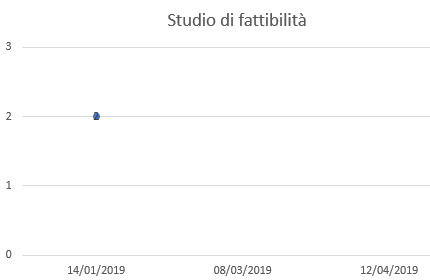
\includegraphics[scale=1]{images/resoconto/Studio.png}
	\caption{Valori ISO/IEC 15504 - Studio di fattibilità}	
\end{figure}


\begin{figure}[H]
	\centering
	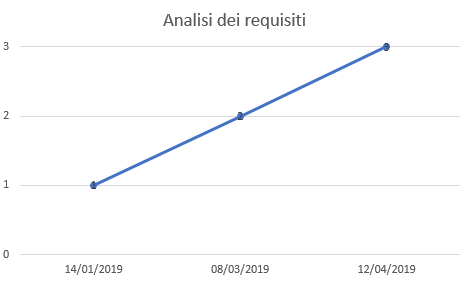
\includegraphics[scale=1]{images/resoconto/Analisi.png}
	\caption{Valori ISO/IEC 15504 - Analisi dei Requisiti}	
\end{figure}


\begin{figure}[H]
	\centering
	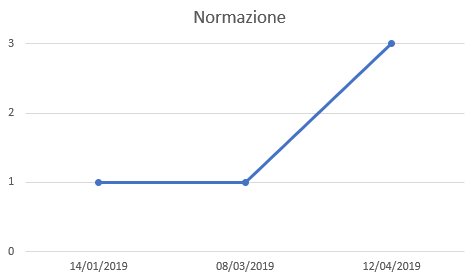
\includegraphics[scale=1]{images/resoconto/Normazione.png}
	\caption{Valori ISO/IEC 15504 - Normazione}	
\end{figure}


\begin{figure}[H]
	\centering
	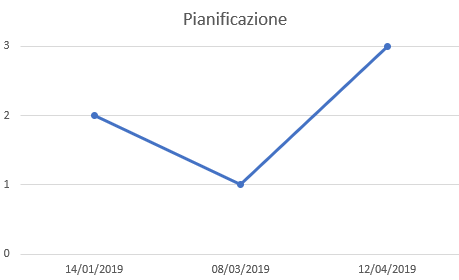
\includegraphics[scale=1]{images/resoconto/Pianificazione.png}
	\caption{Valori ISO/IEC 15504 - Pianificazione}	
\end{figure}


\begin{figure}[H]
	\centering
	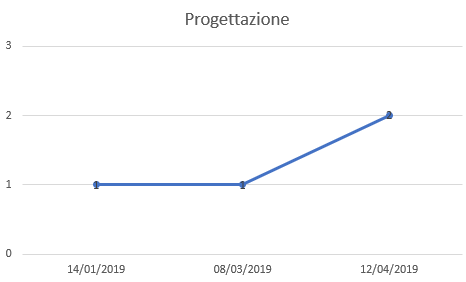
\includegraphics[scale=1]{images/resoconto/Progettazione.png}
	\caption{Valori ISO/IEC 15504 - Progettazione}	
\end{figure}


\begin{figure}[H]
	\centering
	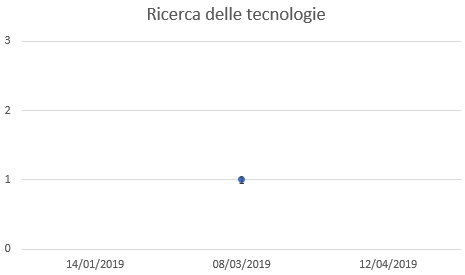
\includegraphics[scale=1]{images/resoconto/Ricerca.png}
	\caption{Valori ISO/IEC 15504 - Ricerca delle tecnologie}	
\end{figure}


\begin{figure}[H]
	\centering
	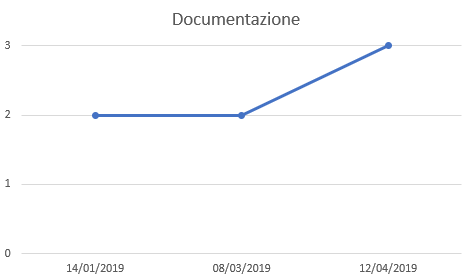
\includegraphics[scale=1]{images/resoconto/Documentazione.png}
	\caption{Valori ISO/IEC 15504 - Documentazione}	
\end{figure}


\begin{figure}[H]
	\centering
	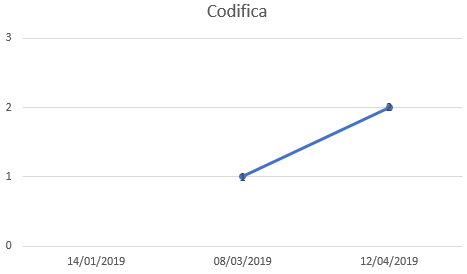
\includegraphics[scale=1]{images/resoconto/Codifica.png}
	\caption{Valori ISO/IEC 15504 - Codifica}	
\end{figure}

\subsubsection{Valori indice RSI - MPC2\\}
Durante lo sviluppo del progetto abbiamo individuato periodicamente tutti i cambiamenti apportati ai requisiti del progetto. Questo ci ha permesso di determinare la stabilità dei requisiti nel tempo grazie all'utilizzo della metrica MPC2.
Riportiamo di seguito i calcoli e le varie rilevazioni effettuate.

\begin{longtable}{>{\centering\arraybackslash}m{3cm} >{\centering\arraybackslash}m{4cm} >{\centering\arraybackslash}m{5cm} >{\centering\arraybackslash}m{2cm}}
	\rowcolor{LightBlue}
	\textbf{\textcolor{white}{Data rilevazioni}}
	& \textbf{\textcolor{white}{Requirement Stability Index (RSI)}}
	& \textbf{\textcolor{white}{Esito}}\\
	
	2019-02-15 & \[1-\frac{0+5+4}{48}=0.81\] & Accettato\\
	\hline
	2019-02-20 & \[1-\frac{5+0+3}{43}=0.81\] & Accettato\\
	\hline
	2019-02-21 & \[1-\frac{8+0+3}{48}=0.77\] & Accettato\\
	\hline
	2019-02-22 & \[1-\frac{5+2+0}{56}=0.85\] & Accettato\\
	\hline
	2019-02-25 & \[1-\frac{11+0+0}{59}=0.81\] & Accettato\\
	\hline
	2019-02-27 & \[1-\frac{10+0+0}{70}=0.88\] & Accettato\\
	\hline
	2019-03-04 & \[1-\frac{12+0+0}{80}=0.86\] & Accettato\\
	\hline
	2019-03-05 & \[1-\frac{14+0+1}{92}=0.83\] & Accettato\\
	\hline\\
	\caption{Rilevazioni indice stabilità requisiti (RSI) - Revisione di progetto}
\end{longtable}
\begin{figure}[H]
	\centering
	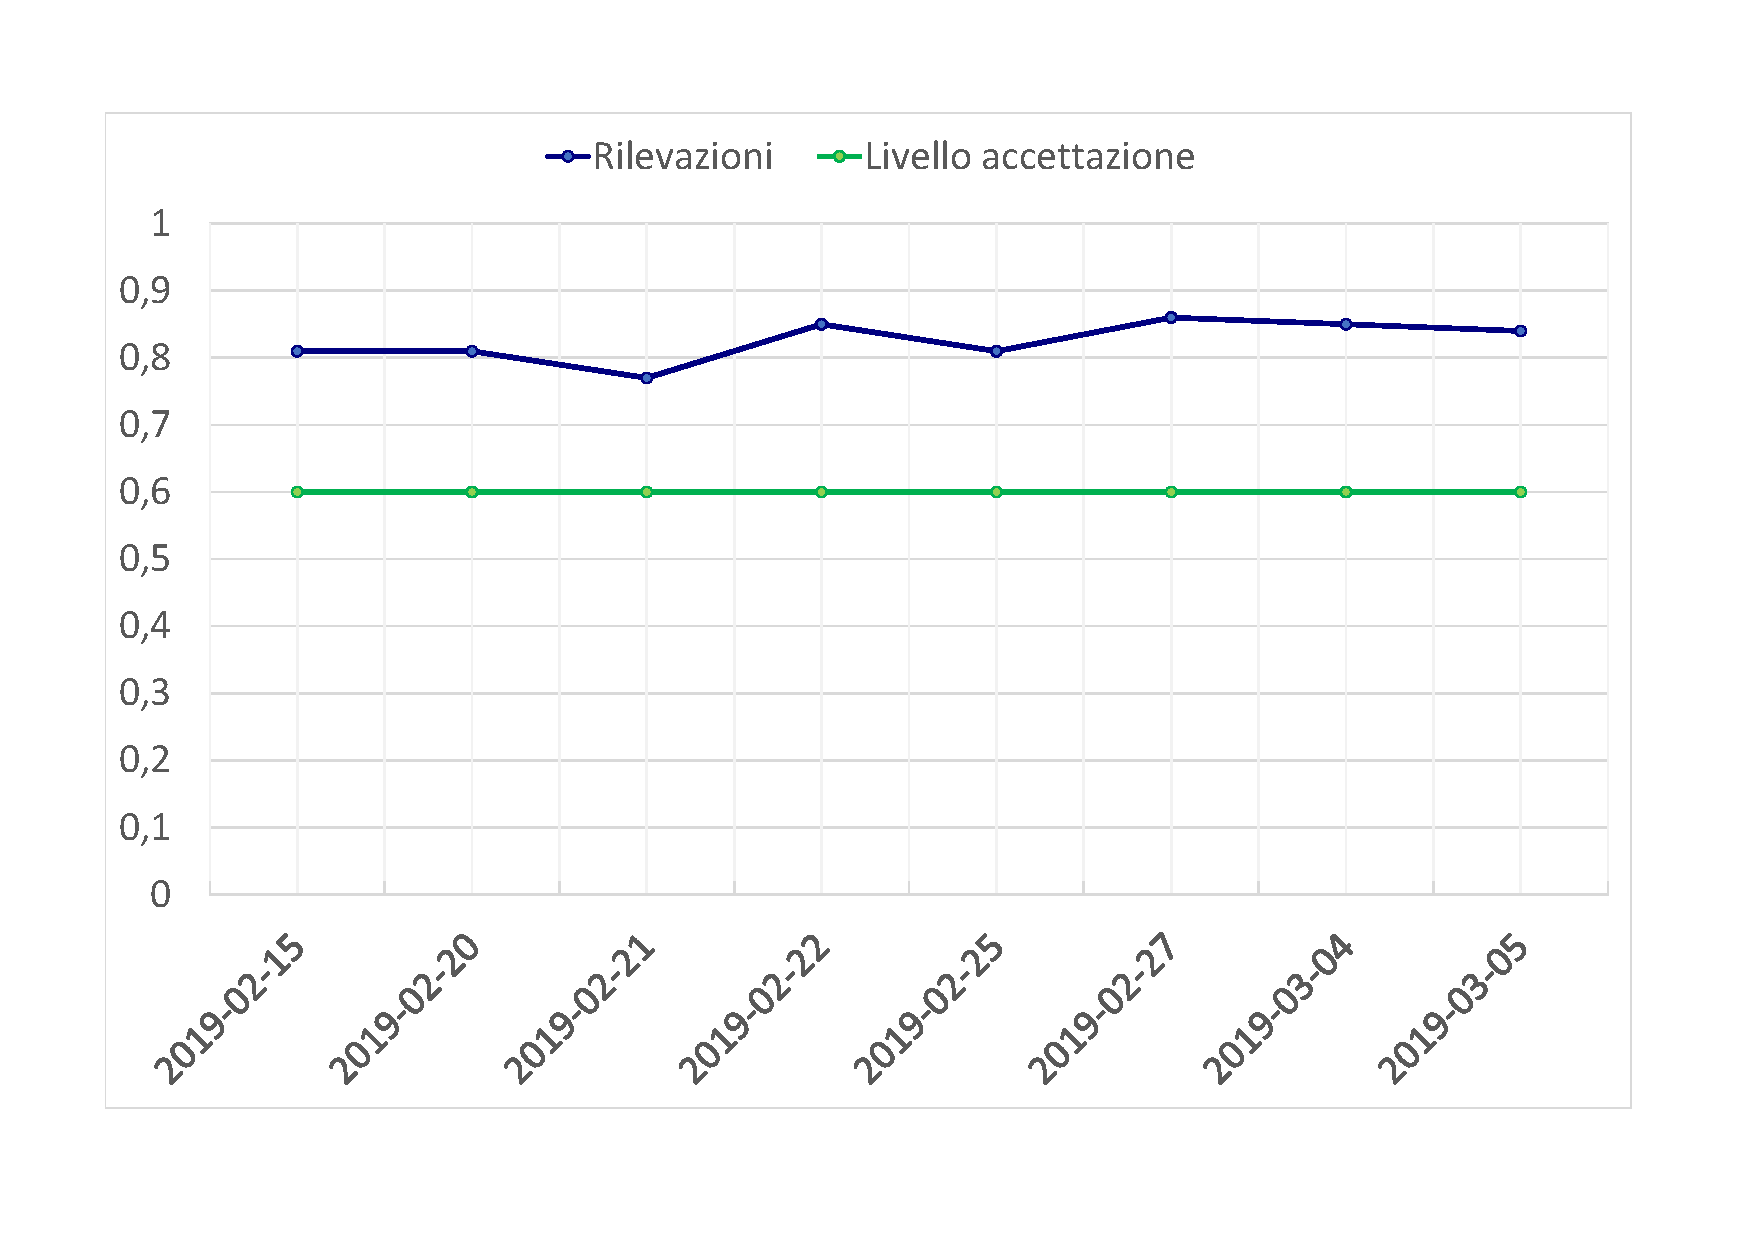
\includegraphics[scale=0.6]{images/resoconto/requisitiChart.pdf}
	\caption{Serie storica rilevazioni stabilità requisiti - Revisione di progetto}	
\end{figure}



\begin{longtable}{>{\centering\arraybackslash}m{3cm} >{\centering\arraybackslash}m{4cm} >{\centering\arraybackslash}m{5cm} >{\centering\arraybackslash}m{2cm}}
	\rowcolor{LightBlue}
	\textbf{\textcolor{white}{Data rilevazioni}}
	& \textbf{\textcolor{white}{Requirement Stability Index (RSI)}}
	& \textbf{\textcolor{white}{Esito}}\\
	
	2019-03-18 & \[1-\frac{9+0+0}{106}=0.915\] & Accettato\\
	\hline
	2019-03-19 & \[1-\frac{13+0+2}{115}=0.869\] & Accettato\\
	\hline
	\caption{Rilevazioni indice stabilità requisiti (RSI) - Revisione di qualifica}
\end{longtable}
\begin{figure}[H]
	\centering
	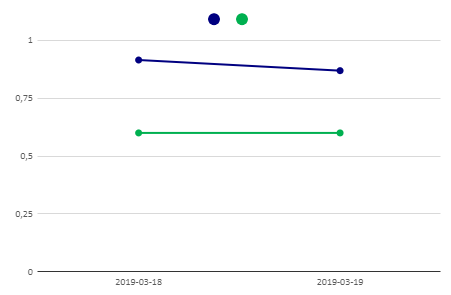
\includegraphics[scale=1]{images/resoconto/qualificaChart.png}
	\caption{Serie storica rilevazioni stabilità requisiti - Revisione di qualifica}	
\end{figure}

\subsection{Esito delle revisioni - RR}
Successivamente alla prima revisione formale, il gruppo ha apportato diverse modifiche ai documenti basandosi sulle osservazioni ricevute dai docenti. Le modifiche sono riassunte di seguito:
	\begin{itemize}
		\item \textbf{Norme di Progetto}: è stata aggiunta una sezione riportante le metriche di riferimento per processi e prodotti e la relativa normazione. 
		\item \textbf{Piano di Progetto}: le attività sono state ripianificate a partire dalla fase 2 ed è stato redatto un nuovo consuntivo.
		\item \textbf{Piano di Qualifica}: la struttura del documento è stata completamente rivista, i contenuti sono stati modificati secondo le indicazioni riportate nell'esito della prima revisione. Sono stati aggiunti diversi tipi di test e diverse appendici con argomenti vari; sono stati stabiliti degli obiettivi di qualità.
		\item \textbf{Analisi dei Requisiti}: sono stati aggiunti diversi nuovi casi d'uso, specializzando quelli già presenti e raddoppiandone il numero; sono stati modificati i diagrammi UML. \`E stata aggiunta una sezione introduttiva ed una descrizione degli attori implicati nel progetto. 
	\end{itemize}

\subsection{Esito delle revisioni - RP}	
Successivamente alla seconda revisione formale, il gruppo ha apportato diverse modifiche ai documenti basandosi sulle osservazioni ricevute dai docenti. Le modifiche sono riassunte di seguito:
	\begin{itemize}
		\item \textbf{Norme di Progetto}: sono state aggiunte diverse norme ed attività al processo di fornitura, revisionando contestualmente quelle già inserite. Sono state rimosse le soglie associate ad ogni metrica e la struttura del documento è stata in parte rivisitata.
		\item \textbf{Piano di Progetto}: le fasi 3 e 4 sono state ripianificate sulla base del periodo precedente; si è cercato di dare maggiore spessore all'incrementalità della logica di sviluppo adottata. 
		\item \textbf{Piano di Qualifica}: la struttura del documento è stata revisionata, sono stati redatti i test di unità e si è cercato di dare una struttura a cruscotto ai riscontri di verifica.
		\item \textbf{Analisi dei Requisiti}: i casi d'uso sono stati rivisti, aumentandone quanto possibile il livello di dettaglio; i codici dei casi d'uso e dei requisiti sono stati modificati e, di conseguenza, hanno subito modifiche anche i diagrammi UML.
	\end{itemize}

\newpage
\section{Copertura dei requisiti}
Viene riportata in seguito una tabella riassuntiva dei requisiti che non è da considerarsi definitiva, verrà infatti aggiornata in seguito ad ogni avanzamento significativo. \\
I requisiti sono indicati con il loro codice identificativo definito nel documento \textit{NormeDiProgetto\_v3.0.0} e la loro descrizione dettagliata è riportata nel documento \textit{AnalisiDeiRequisiti\_v3.0.0}.
\begin{longtable}{| p{2.5cm} | p{3cm} |}
	\rowcolor{LightBlue}
	\color{white}\bfseries Requisito & \color{white}\bfseries Stato \\
	ROF1 & Soddisfatto \\ \hline
	ROF2 & Soddisfatto \\ \hline
	ROF3 & Soddisfatto \\ \hline
	ROF4 & Soddisfatto \\ \hline
	ROF5 & Soddisfatto \\ \hline
	ROF6 & Soddisfatto \\ \hline
	ROF7 & Soddisfatto \\ \hline
	ROF8 & Soddisfatto \\ \hline
	ROF9 & Soddisfatto \\ \hline
	ROF10 & Soddisfatto \\ \hline
	ROF11 & Soddisfatto \\ \hline
	ROF12 & Soddisfatto \\ \hline
	ROF13 & Soddisfatto \\ \hline
	ROF14 & Soddisfatto \\ \hline
	ROF15 & Soddisfatto \\ \hline
	ROF16 & Soddisfatto \\ \hline
	ROF17 & Soddisfatto \\ \hline
	ROF18 & Soddisfatto \\ \hline
	ROF19 & Soddisfatto \\ \hline
	ROF20 & Soddisfatto \\ \hline
	ROF21 & Soddisfatto \\ \hline
	ROF22 & Soddisfatto \\ \hline
	ROF23 & Soddisfatto \\ \hline
	ROF24 & Soddisfatto \\ \hline
	ROF25 & Soddisfatto \\ \hline
	ROF26 & Soddisfatto \\ \hline
	ROF27 & Soddisfatto \\ \hline
	ROF28 & Soddisfatto \\ \hline
	ROF29 & Soddisfatto \\ \hline
	ROF30 & Non soddisfatto \\ \hline
	ROF31 & Non soddisfatto \\ \hline
	ROF32 & Non soddisfatto \\ \hline
	ROF33 & Soddisfatto \\ \hline
	ROF34 & Non soddisfatto \\ \hline
	ROF35 & Non soddisfatto \\ \hline
	ROF36 & Non soddisfatto \\ \hline
	ROF37 & Non soddisfatto \\ \hline
	ROF38 & Non soddisfatto \\ \hline
	ROF39 & Non soddisfatto \\ \hline
	RDF1 & Soddisfatto \\ \hline
	RDF2 & Soddisfatto \\ \hline
	RDF3 & Soddisfatto \\ \hline
	RDF4 & Soddisfatto \\ \hline
	RDF5 & Non soddisfatto \\ \hline
	RDF6 & Non soddisfatto \\ \hline
	RDF7 & Soddisfatto \\ \hline
	RDF8 & Soddisfatto \\ \hline
	RDF9 & Soddisfatto \\ \hline
	RDF10 & Non soddisfatto \\ \hline
	RDF11 & Non soddisfatto \\ \hline
	RDF12 & Non soddisfatto \\ \hline
	RDF13 & Non soddisfatto \\ \hline
	RDF14 & Non soddisfatto \\ \hline
	RDF15 & Non soddisfatto \\ \hline
	RDF16 & Non soddisfatto \\ \hline
	RDF17 & Non soddisfatto \\ \hline
	RDF18 & Non soddisfatto \\ \hline
	RDF19 & Non soddisfatto \\ \hline
	RDF20 & Non soddisfatto \\ \hline
	RDF21 & Non soddisfatto \\ \hline
	RDF22 & Non soddisfatto \\ \hline
	RDF23 & Non soddisfatto \\ \hline
	RDF24 & Non soddisfatto \\ \hline
	RDF25 & Non soddisfatto \\ \hline
	RDF26 & Non soddisfatto \\ \hline
	RDF27 & Non soddisfatto \\ \hline
	RDF28 & Non soddisfatto \\ \hline
	RDF29 & Non soddisfatto \\ \hline
	RDF30 & Non soddisfatto \\ \hline
	RDF31 & Non soddisfatto \\ \hline
	RDF32 & Non soddisfatto \\ \hline
	RDF33 & Non soddisfatto \\ \hline
	RDF34 & Non soddisfatto \\ \hline
	RDF35 & Non soddisfatto \\ \hline
	RDF36 & Non soddisfatto \\ \hline
	RDF37 & Non soddisfatto \\ \hline
	RDF38 & Non soddisfatto \\ \hline
	RDF39 & Non soddisfatto \\ \hline
	RDF40 & Non soddisfatto \\ \hline
	RDF41 & Non soddisfatto \\ \hline
	RDF42 & Non soddisfatto \\ \hline
	RDF43 & Non soddisfatto \\ \hline
	RDF44 & Non soddisfatto \\ \hline
	RPF1 & Non soddisfatto \\ \hline
	RPF2 & Non soddisfatto \\ \hline
	RPF3 & Non soddisfatto \\ \hline
	RPF4 & Non soddisfatto \\ \hline
	RPF5 & Non soddisfatto \\ \hline
	RPF6 & Non soddisfatto \\ \hline
	RPF7 & Non soddisfatto \\ \hline
	RPF8 & Non soddisfatto \\ \hline
	RPF9 & Non soddisfatto \\ \hline
	RPF10 & Non soddisfatto \\ \hline
	RPF11 & Non soddisfatto \\ \hline
	RPF12 & Non soddisfatto \\ \hline
	RPF13 & Non soddisfatto \\ \hline
	RPF14 & Non soddisfatto \\ \hline
	RPF15 & Soddisfatto \\ \hline
	RPF16 & Soddisfatto \\ \hline
	RPF17 & Non soddisfatto \\ \hline
	RPF18 & Non soddisfatto \\ \hline
	RPF19 & Non soddisfatto \\ \hline
	RPF20 & Non soddisfatto \\ \hline
	RPF21 & Non soddisfatto \\ \hline
	RPF22 & Non soddisfatto \\ \hline
	RPF23 & Non soddisfatto \\ \hline
	RPF24 & Non soddisfatto \\ \hline
	RPF25 & Non soddisfatto \\ \hline
	RPF26 & Non soddisfatto \\ \hline
	RPF27 & Non soddisfatto \\ \hline
	RPF28 & Non soddisfatto \\ \hline
	RPF29 & Non soddisfatto \\ \hline
	RPF30 & Non soddisfatto \\ \hline
	ROV1 & Soddisfatto \\ \hline
	ROV2 & Soddisfatto \\ \hline
	ROV3 & Soddisfatto \\ \hline
	ROV4 & Soddisfatto \\ \hline
	RDV1 & Soddisfatto \\ \hline
	RPV1 & Non soddisfatto \\ \hline
	ROQ1 & Soddisfatto \\ \hline
	ROQ2 & Soddisfatto \\ \hline
	ROQ3 & Soddisfatto \\ \hline
	RDQ1 & Soddisfatto \\ \hline
	RDQ2 & Non soddisfatto \\ \hline
	RDQ3 & Soddisfatto \\ \hline
	RDQ4 & Non soddisfatto \\ \hline
	RDQ5 & Non soddisfatto \\ \hline
	RPQ1 & Non soddisfatto \\ \hline
	\caption{Riassunto copertura requisiti}
\end{longtable}


	
